\chapter{Literature Study}
In this chapter research is conducted to determine the viability and 


\section{History}
\subsection{Micro Aerial Vehicles}
Flight has long been a phenomenon man has attempted to harness and understand. There are numerous methods of obtaining flight and these all come with their own advantages and disadvantages. As technologies advance they have a tendency to scale down in size, cost and complexity. In the realm of aerial vehicles this has resulted in the development of various micro aerial vehicles, or MAVs \cite{Leishman}. Having significantly lower Reynold's numbers than traditional big aircraft meant that the flow characteristics of these designs would differ. These small craft represent both a technology challenge and a potential new vehicle class that may have substantial societal impact" \cite{NewMAV}

In the realm of MAVs the rotor winged craft brings certain advantages to the table. For environments were high levels of manoeuvrability are required, or even a situation where the platform might need to remain still a rotary design should be considered \cite{Bohorquez}


Specifying that the robot must work in a close quarter environment limits the choice of drive systems \cite{CQAR}. 
For example a fixed wing aircraft would not be a feasible design due to the lack of manoeuvrability and inability to hover. The limited control behind a ducted fan design limits the usefulness in more delicate missions. Due to space requirements in the design specifications, lighter than air vehicles (such as blimps) have not been considered.

This leaves a rotor wing design which is discussed in detail below. The modern day rotor wing aircraft plays a unique role in new age aviation \cite{Leishman} and is required in an application where the platform might need to stand still \cite{Bohorquez}. 

\todo[inline]{When more theory is applicable must add to this section}


%RESEARCH INTO ROTOR THEORY

\section{Flight Theory}
Flight is a broad term and can be seen from as simple a concept as hot smoke rising to a bird flapping its wings. The reality is that flight even encompasses a rugby ball, kicked by Joel Stransky, flying through the air to win South Africa the Rugby World Cup. Although all different forms of flight, the examples above will have a very similar force diagram as seen in figure \ref{IM_FlightForces}.

\begin{figure}
\centering
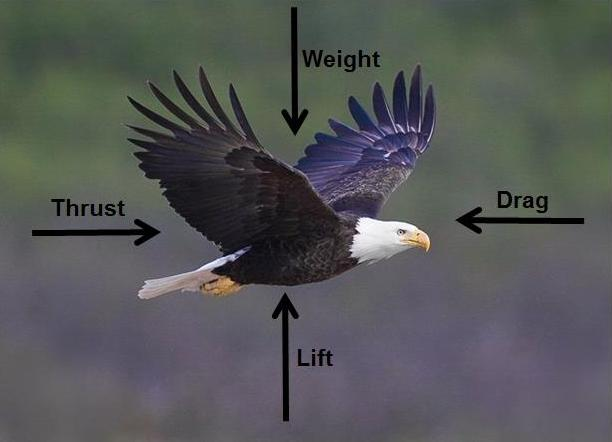
\includegraphics[height = 6cm]{Images/Literature/Bird}
\caption{Force diagram of basic components of flight (Picture adapted from National Geographic Website)}
\label{IM_FlightForces}
\end{figure}

From the force diagram it can be intuitively seen that to increase the velocity of a body in air, the lift must exceed the weight. Kevin Sablan gives a good summary of the forces in \cite{TheoryofFlight}.
Weight is directly determined by the object's mass and the relevant gravity coefficient, $W = mg$. Lift counteracts this weight in an attempt to boost the body into the air. Upward acceleration is only achieved once lift exceeds weight, if they are equal the body will be in a state of hover. From the lift equation seen in equation \ref{EQ_Lift} only a body with velocity can obtain lift. In a rotorcraft, like a helicopter, the rotating blades move through the air and generate lift, the amount generated is governed by equation \ref{EQ_Lift}. 

As seen in figure \ref{IM_Helicopter} the main rotor system, which consists of these rotating blades, is directly coupled to the fuselage and the entire vehicle is lifted into the air. In a fixed wing aircraft if the vehicle is stationery, according to the equation, lift must be zero as there are no moving components. 

\begin{equation}
\label{EQ_Lift}
Lift = C_L(\frac{1}{2} \rho V^2) S
\end{equation}

To propel the body forward the thrust must exceed the value of the drag force acting directly against its velocity vector. Thrust is calculated by combining multiple fields of physics, the effect of thrust can be best summarised by Newton's second law of motion, $F=ma$. The force is generated through interaction with the surrounding atmosphere. Newton's third law agrees that by accelerating large masses of air, thrust is generated in the opposite direction. In the case of a gliding bird, the thrust will equal to zero and the bird will gradually slow down until it flaps its wings again to produce more thrust. This loss of speed is due to drag. Similar to lift, drag varies with velocity as shown in equation (\ref{EQ_Drag}).

\begin{equation}
\label{EQ_Drag}
Drag = C_D (\frac{1}{2} \rho V^2) A
\end{equation}

The coefficient of drag ($C_D$) is determined by the way the object interacts with the air flow, this will comprise of smoothness values as well as shape. 


\subsection{Fundamental Principles of Flow}
Flow is created by any body moving through a medium be it air, water or sand. Therefore any object with an airborne trajectory will be in part governed by the laws of flow. To better understand the principles behind flight, certain theories of flow must be understood.

\subsubsection{Continuity Equation and Bernoulli's Principle}
The continuity equation is used in varying fields of study, it dictates the behaviour of certain phenomenon, or better said their ability to not change. Daniel Bernoulli observed that the mass flow of a flowing medium will follow the laws of continuity in the form of equation \eqref{EQ_Bernoulli}. To do this he observed the conservation of mass flow in a closed system, as shown in equation \eqref{EQ_BernoulliP}. This principle states that in a closed system, the product of density ($\rho$), area (A) and velocity (v) for a flowing system will remain constant \cite{Dayle}. Bernoulli then elaborated on the above statements and wanted to determine how the pressure of the system will affect the mass flow. Since $P = \frac{F}{A}$, it can be seen that pressure will directly affect the flow rate.

\begin{equation}
\label{EQ_BernoulliP}
\rho Av = Constant
\end{equation} 

The Bernoulli equation is a statement of the conservation of energies present in a flowing system \cite{Dayle}. Equation \ref{EQ_Bernoulli} considers a pipe with a flowing liquid and states that the energy in the system will remain unchanged in a closed system. The sum of these energies will contain the kinetic energy of the liquid as well as the pressure energy. Bernoulli's equation takes these principles and allows the manipulation of certain variables to create lasting effects on other ones.

\begin{eqnarray}
P_0 + \frac{1}{2} \rho v_0^2 &=& P_1 + \frac{1}{2} \rho v_i^2\label{EQ_Bernoulli}\\
P_2 - P_1 &=& \frac{1}{2} \rho (v_\infty^2 - v_0^2)\label{EQ_Bernoulli2}
\end{eqnarray}

\subsubsection{Reynold's Number}
Moving different objects in the same environment will create different results of flow, in the same breath moving the same object through different environments will also create various results of flow. Osborne Reynold attempted to mathematically determine these effects and quantify what caused a system to have turbulent flow opposed to laminar flow and vice versa. During his research he created a dimensionless constant known as the Reynold's number, as shown in equation \ref{EQ_Reynold} \cite{Reynold}. 

\begin{equation}
\label{EQ_Reynold}
Re = \frac{\rho v L}{\mu}
\end{equation} 

In its simplest form, the Reynold's number of an object is the ratio between inertial forces ($\rho v L$) and viscous forces ($\mu$) of the gas. In a system where the viscous forces dominate ($Re ~< 10^3$), there will be laminar flow and when there are higher inertial forces ($Re >~ 10^4$) the flow will be turbulent. In layman's terms, if the disruptive forces (inertial) are much greater than the forces keeping the gas together (viscous), the flow will be turbulent. 
Since turbulent flow will decrease stability and increase drag forces, Reynold's numbers have become a very important part in correctly modelling and designing aircraft \cite{Reynold}.


\subsection{Basic Rotor Theory}
The understanding behind rotor aerodynamics is a constantly on going discussion, with recent developments relating in significant gains of helicopter performance. The rotor is responsible for all the aspects of flight and generates the lift, forward propulsion and the means to control the orientation of the craft \cite{Leishman}. It is for this reason that an in depth understanding of rotor characteristics and performance was done. The original research into rotor analysis was done with helicopters, but the rotor theory basics are relevant to any rotating winged craft.

Due to Newton's third law, any rotating blade will cause a a rotation in the opposite direction to that motion. This applied force will drive the vehicle to rotate around that spinning axis and creates the need for a counter torque mechanism. This is common with most rotorcraft and can be visualised in figure \ref{IM_Antitorque}, in the form of the tail rotor as seen in conventional helicopters.

\begin{figure}[H]
\centering
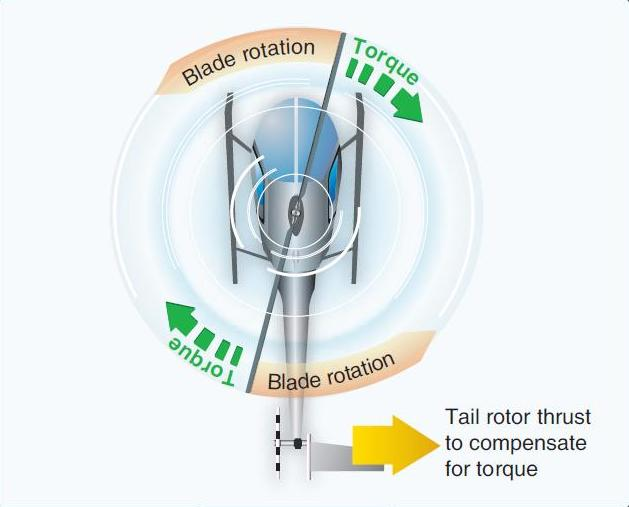
\includegraphics[height = 6cm]{Images/Literature/AntiTorque}
\caption{Image Illustrating generation of Counter Torque (Taken from \cite{Heli})}
\label{IM_Antitorque}
\end{figure}

The capability of any part of a rotor to produce lift is influenced by the local blade position and pressure at that point \cite{Leishman}.
As the rotor spins, the blade's angle of attack shifts. This angle is defined as an azimuth angle ($\psi$) and is measured relative to air flow. The azimuth angle is 0\textdegree down stream and sits at 180\textdegree when it faces directly upstream.
Angular velocity equations state that the speed of any part of the rotor varies along the length of the rotor. With the maximum velocity sitting at the rotor tip. As the rotorcraft adds a horizontal component to its hover or vertical flight, the relative speed of the individual rotor segments now adheres to equation \eqref{EQ_TipSpeed}. As visualised in figure \ref{IM_TipSpeed}, the relative velocity at the any part of the rotor is affected by the azimuth angle of the blade ($\psi$), forward translatory speed of the craft ($V_{\infty}$), angular speed of the rotor ($\Omega$) and the considered distance along the rotor blade (r) \cite{Leishman} \cite{RotorCraftHand}. 

\begin{equation}
\label{EQ_TipSpeed}
V_{r} = \Omega r + V_{\infty}\sin(\psi)
\end{equation}

\begin{figure}[h]
\centering
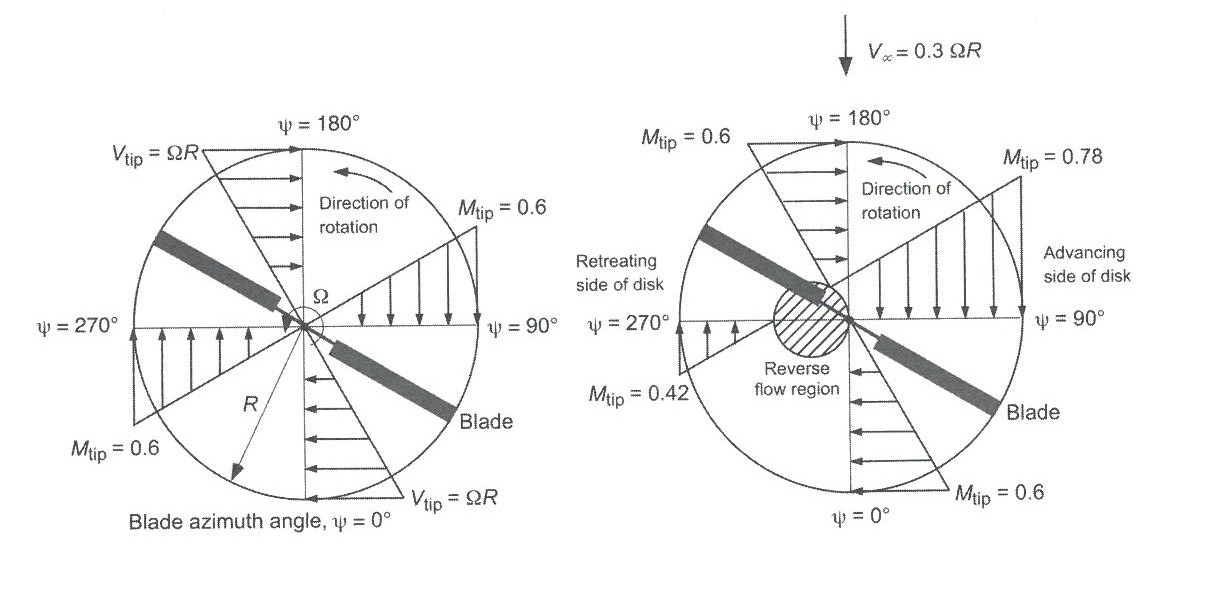
\includegraphics[height = 6cm]{Images/Literature/TipSpeed}
\caption{Velocity components of a rotor \cite{Leishman}}
\label{IM_TipSpeed}
\end{figure}

What this relationship shows is that during forward flight the tip velocity, relative to the ground, changes even if the rotor rotates at a constant speed. This complicates the rotor dynamics at higher speeds and limits the top speed of the craft. On the retreating edge ($\psi = 270$\textdegree $\therefore sin(\psi) = -1$) if $\Omega r <= V_{\infty}$ the rotor would effectively be going backwards and the helicopter is at risk of stalling out, this is known as a stall condition \cite{Leishman} \cite{RotorCraftHand}, while the advancing edge is reaching its maximum speed by approaching Mach conditions and sever instability.

\subsection{Momentum Theory and Thrust Basics}

As mentioned above the rotors of a rotorcraft are responsible for generating all the forces that manoeuvre the vehicle. These forces are induced by pushing air through the rotor disk. With a fixed wing aircraft the analysis of the blades is simplified because the only air flow produced is from the translational velocity of the entire craft. Analysis of blade performance in a rotorcraft can be more challenging as the rotation of the blades must be considered along side the overall speed of the vehicle. As the craft manoeuvres in space, the air flow through the rotor has significant complexities which complicates the analysis. Since the rotorcraft is expected to perform in a variety of flight styles it is important to understand these models, and their flaws. 

To simplify, initially consider a helicopter in a hovering state (Weight(W) = Thrust(T)). Figure \ref{IM_MomentumTheoryAirFlow}, taken from \cite{Leishman}, helps visualise the induced air flow by showing how the rotor smooths out the air by forcing it through the disk area. This more uniform air creates an edge known as the slipstream or wake boundary, with the surrounding air remaining dormant \cite{Leishman}. Inside the wake boundary, the average velocity of the air is tangible and effective, where outside the slipstream edge, the average air velocity is negligible and obsolete. The force required to push that mass of air through the disk space is, by Newton's third law, returned by the air unto the rotor. Thus giving the rotor blades a thrust component.
  
\begin{figure}[h]
\centering
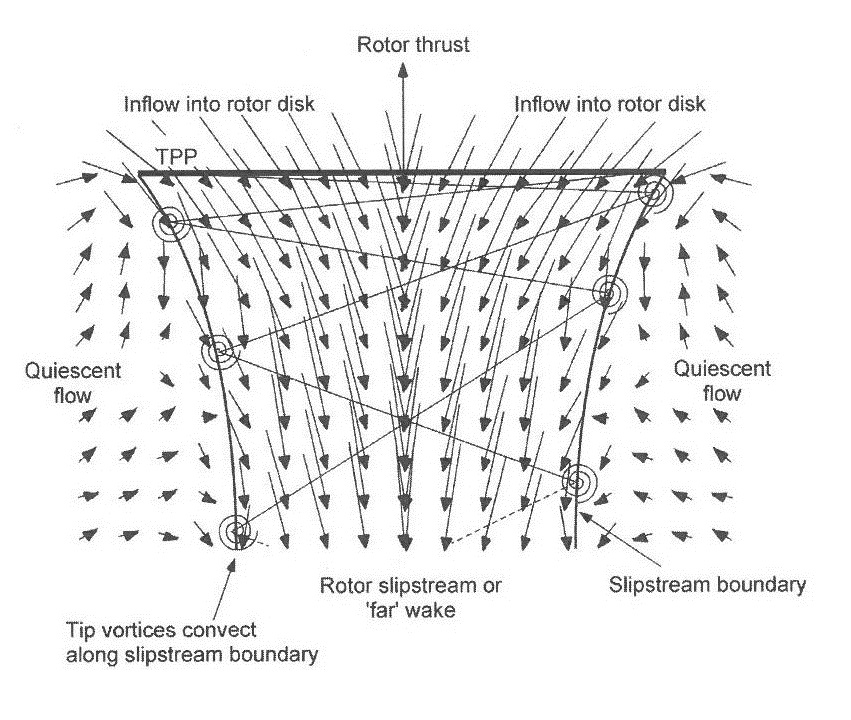
\includegraphics[height = 8cm]{Images/Literature/MomentumTheoryAirFlow}	
\caption{Visualisation of Induced Air Flow Through A Rotor \cite{Leishman}}
\label{IM_MomentumTheoryAirFlow}
\end{figure}

Rankine-Froude's Momentum Theory looks at this induced velocity as well as the displacement of air through the propeller, and attempts to quantify the induced thrust. While figure \ref{IM_MomentumTheoryAirFlow} helps visualise the principle, the variable naming convention for the equations is shown in figure \ref{IM_MomentumTheoryHover} below. 
Labels 0, 1, 2 and $\infty$ refer to the locations of quiescent flow, inflow directly before the rotor, airflow immediately after the disk and the slipstream\footnote{Generally far wake is considered as 1 full rotor diameter distance away \cite{Leishman}.} or far wake condition respectively.
The velocities are shown as the induced velocity in and out the rotor ($v_{i}$), the far wake velocity ($v_{\infty}$) and finally $v_{0}$ represents the zone with zero flow rate. There is no velocity jump across the rotor, the energy being fed into the system by the rotor is represented by a pressure change.

\begin{figure}[h]
\centering
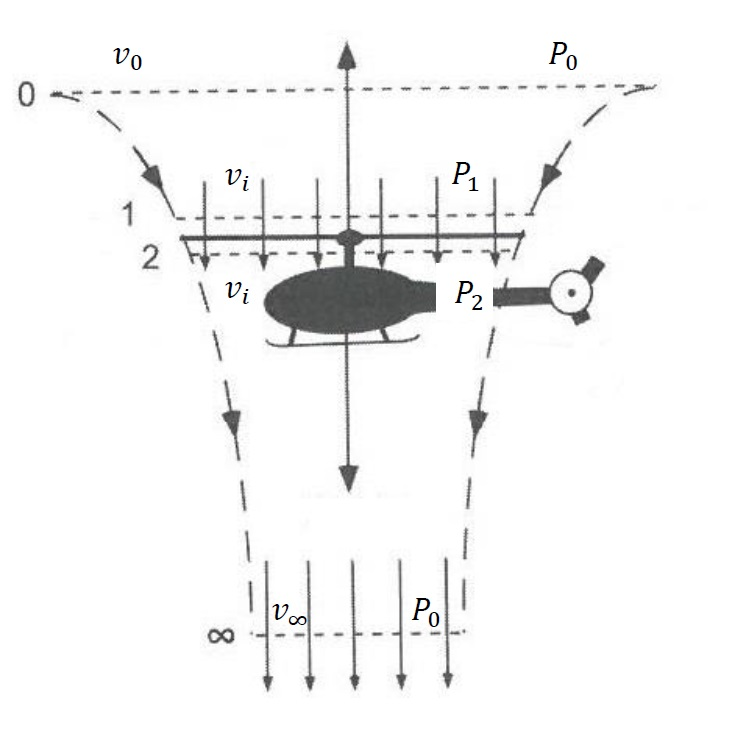
\includegraphics[height = 8cm, angle=360]{Images/Literature/MomentumTheoryHover}			%Must show both air flow as well as far stream and such
\caption{Momentum Theory in Hover (Adapted From \cite{Leishman})}
\label{IM_MomentumTheoryHover}
\end{figure}

As described above, it is by forcing the air through the disk that lift is generated. The mass flow rate of this air can then be described by (\ref{EQ_MassFlow}), where ($\rho$) is the density of air and A is the area of one full blade rotation. The rate at which this mass of air is displaced becomes a crucial variable in rotor dynamics and is directly proportional to thrust (T). This relationship can be quantified as shown in (\ref{EQ_ThrustBasic}). Thrust can also be calculated by finding the difference in pressures over the rotor disk as in (\ref{EQ_ThrustPressure})

\begin{eqnarray}
\dot{m} &=& \rho A v_{i}\label{EQ_MassFlow}\\
T &=& \dot{m}a\label{EQ_ThrustBasic}\\
T &=& A(P_2 - P_1)\label{EQ_ThrustPressure}
\end{eqnarray}

Since $v_0$ is zero during hover and acceleration is the difference in $v_\infty$ and $v_0$, equation (\ref{EQ_ThrustMass}) can be obtained.

\begin{equation}
\label{EQ_ThrustMass}
T = \rho A v_{i} v_\infty
\end{equation}

Thrust can now be quantified if the slipstream and induced velocities are known. 
Then by applying Bernoulli's equation of conservation (\ref{EQ_Bernoulli}) to both sides of the rotor disk, the change in pressure across the disk can be quantified as shown in (\ref{EQ_Bernoulli2}).
That change in pressure fits into one of the initial definitions of thrust (\ref{EQ_ThrustPressure}). Equating both of those definitions yields an important relationship between the three velocities, as shown in (\ref{EQ_RotorVelocity}). The relationship simply states that the induced velocity at the rotor is the average of the quiescent flow above and the far wake velocities. This definition proves useful at a later stage in the rotor theory definitions. 

\begin{equation}
\label{EQ_RotorVelocity}
v_i = \frac{1}{2} (v_\infty + v_0)
\end{equation}

\subsection{Disk and Power Loading}
\subsubsection{Disk Loading}
Disk loading (DL) is a term seen often in the world of rotorcraft, it is a simple but important ratio between thrust and the area a rotating disk makes.  It is represented in its simplest form in the beginning of equation \eqref{EQ_DL}. Since the pressure drop across each rotor is considered uniform, the disk loading for each rotor will equate to the pressure drop across that disk. Equation (\ref{EQ_Bernoulli2}) first shows the difference in pressure and by taking $v_0$ as zero, the second half of equation (\ref{EQ_DL}) can be formed. 
\begin{equation}
\label{EQ_DL}
DL (\frac{N}{m^{2}})= \frac{T}{A} = \frac{1}{2} \rho v_\infty^2
\end{equation}

For multi-rotor craft, the disk loading is assumed uniform across all rotors \cite{Leishman}. The overall disk loading of a single rotorcraft such as a traditional helicopter will be lower than that of a multi-rotor craft of a similar size \cite{RotorCraftHand}.  Figure \ref{IM_DL} shows some examples of disk loading values for a variety of rotor configurations, as shown disk loading is also a measure of hover efficiency.

\begin{figure}[H]
\centering
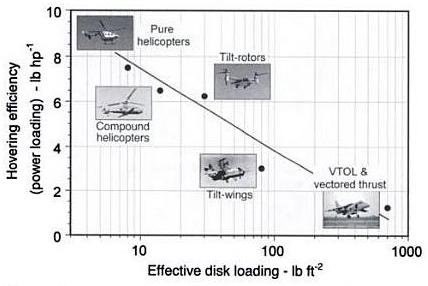
\includegraphics[height = 6cm]{Images/Literature/DL}     
\caption{Image representing, various Disk Loading values for varying rotorcraft (Taken from \cite{Leishman})}
\label{IM_DL}
\end{figure}

A higher disk loading value results in larger values for induced velocities as well as the required power to hover. This means that the larger the blades, the better the efficiency. More force will be generated by pushing large quantities of air slowly, than forcing small amounts of air through at high speeds. Of course with bigger blades, comes larger rotational inertia and geometry as well as the craft being less immune to gusts and interferences. A larger blade also creates faster tip velocities, which will limit the speed of the craft severely \cite{Leishman}.



\subsubsection{Power Loading}
Power is given by the product of both Thrust and the induced velocity at the blade. It can be written as shown in equation (\ref{EQ_Power}). What this ratio shows is that the ideal power is in cubic proportion to the induced velocity at the rotor. Therefore to reduce required power the rotor's induced velocity must be small, which can be accomplished by a significant increase in disk area \cite{Leishman}.

\begin{equation}
\label{EQ_Power}
P = 2 \rho A v_{i}^3
\end{equation}

Another important ratio is between thrust and power, it is called power loading (PL) and is shown in equation (\ref{EQ_PL}). Power loading can be seen as a measure of craft efficiency. 

\begin{equation}
\label{EQ_PL}
PL (\frac{N}{kW})= \frac{T}{P}
\end{equation}

From equations \eqref{EQ_DL} and \eqref{EQ_PL} it can be shown that power loading is inversely proportional to disk loading. Therefore a craft with a lower disk loading will generally be a more efficient platform.

\subsection{Electrical Power to Thrust}
Equation (\ref{EQ_Power}) gives a quantitative approach to solving for aerodynamic power ($P_i$). If electrical power is taken as $P_e = VI$, where V is the applied voltage and I is the sourced current, with an efficiency of $\eta$ then $P_i = \eta VI$. Noting that $P_i = T v_i$ and using equation (\ref{EQ_Power}), a relationship between thrust and $P_e$ can be formed and is represented in equation (\ref{EQ_ElectricalPowerThrust}).

\begin{equation}
\label{EQ_ElectricalPowerThrust}
T = (2\rho A)^{\dfrac{1}{3}} (\eta P_e)^{\dfrac{2}{3}}
\end{equation}

Equation (\ref{EQ_ElectricalPowerThrust}) brings to light a very important relationship which states that thrust grows at a slower rate than the electrical input power to the system.

\begin{equation*}
T \propto P_e^{\dfrac{2}{3}}
\end{equation*}

\section{Analysis of Conventional Rotor Wing Configurations}

Some of the fundamental theories described above relate to the basics behind various rotor configurations and even varying flight techniques. Each different arrangement of blades introduces certain advantages and disadvantages to the system. Not every configuration will be applicable for all operations and it is important to determine what criteria are critical for the intended application.  An analysis of varying rotor configurations is done below and follows a similar trend to that seen in \cite{RotorConfig}, \cite{Bohorquez} and \cite{NewMAV}. The main weighted criterion for the discussion were listed in no particular order as:

\begin{enumerate}
	\item Flight time and efficiency
	\item Geometry and size
	\item Drone Manoeuvrability
	\item Control algorithms
	\item Mechanical complexity
\end{enumerate}

Before the analysis can be done, certain operating parameters of the different craft, surrounding the above mentioned criteria, need to be understood. There has been discussions regarding why and how rotor blades produce lift, this section discusses the real world implementation of those blades.


The same way that a car tyre is the only way the energy from the engine is translated into motion, the rotor in a rotorcraft is responsible for taking the kinetic energy from the motors and translating it into flight. Typically a rotorcraft will be designed with either fixed pitched, or variable pitched rotors. A fixed pitched rotor is a rotor that has an optimally selected, unchangeable pitch and therefore a fixed angle of attack. This of course means that since the angle of attack is fixed for the blade, an increase in speed will be required for a change in lift. With a variable pitched blade, the pilot can change the angle of attack to increase the forces. As the angle of attack increases, the blade will produce more lift without changing the speed of the motor. However, as the pitch increases, so does the drag of the blade. This then requires more motor power to keep the blade moving through the air.
The power requirements for either system are fairly similar, the advantages of a varying pitch is a single rotor has the potential for more dynamic force applications. The downfall however is the high level of complexity in the mechanical design. Both of these facts become pertinent in the final decision making of the platform design.

It is also known that any rotating member will produce a counter rotating torque to the static body, which means that any system with only one rotor will have inherent instability in the yaw axis. The end goal is to have a craft that can fly stably and accurately in 3 dimensions. To do this the craft will need more control surfaces to apply forces in those planes. Figure \ref{IM_PRY}\footnote{http://weboflife.nasa.gov/learningResources/vestibularbrief.htm} shows the planes and the standard naming convention. 

\begin{figure}[H]
	\centering
	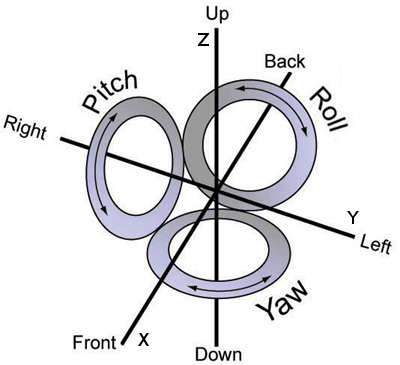
\includegraphics[height = 6cm]{Images/Literature/RollPitchYaw}     
	\caption{Control surfaces required for 3 dimensional flight \cite{Heli})}
	\label{IM_PRY}
\end{figure}

In mathematics discussions are had regarding rotations around the x, y and z axes, in flight theory they are labelled as roll, pitch and yaw. The three axes change as the aircraft changes since they are labelled relative to the aircraft's position. Pitch relates to how much the vehicle is tipping forward or backward, roll is an influence in the left and right rotation, while yaw is rotation around the z axis. Instead of  x, y and z, these axes can be considered as forward, sideways and vertical \cite{Leishman}.

Having only a single, fixed pitched rotor allows only for control in the amount the craft flies up or down, as well as this fore mentioned instability. There are many different methods to obtain full six degrees of flight freedom. The following discussion tries to address each point listed above for each different method, while trying to achieve an optimised design.


\subsection{Helicopter}
When most people think of a rotorcraft they will think of a conventional helicopter, which is still the most widely used configuration for large rotorcraft \cite{RotorConfig}. It consists of a single main rotor, coupled with a smaller counter rotating rotor located in the tail as seen in figure \ref{IM_Helicopter}\footnote{(Adapted from \cite{Heli})}, this is to counteract the developed counter torque as shown in figure \ref{IM_Antitorque}.

\begin{figure}[H]
\centering
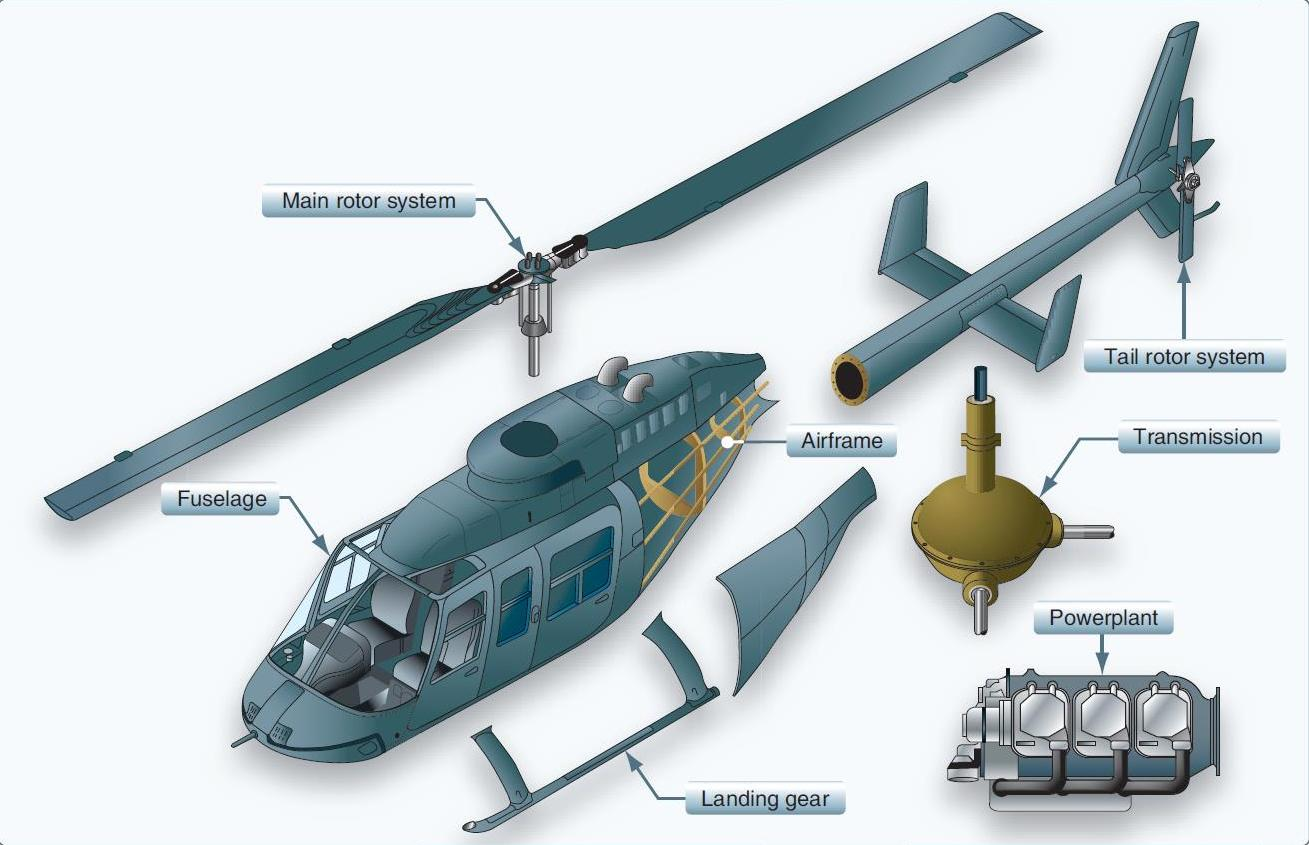
\includegraphics[height = 6cm]{Images/Literature/MainHeliComponents}     
\caption{Main Components of a helicopter \cite{Heli}}
\label{IM_Helicopter}
\end{figure}

The main rotor of a standard helicopter has very low disk loading which gives it excellent hover efficiency. Since the desired end product will mostly be in a state of hover or at least slow lateral movement, this will yield good results for flight time. To achieve yaw stability this configuration makes use of a small tail rotor to counter act the induced moments. The extended tail rotor requires energy which it will draw from the motor while also adding a significant amount of length to the craft. Since the single rotor only gives the pilot thrust control and the tail rotor gives measurable yaw control, there is need for more control surfaces to do more manoeuvring. To implement this most helicopters use a variable pitched rotor system. Cyclic control of this pitch allows the pilot to adjust the angle of attack of the rotor blades while they rotate, thus a forward pitch can be applied by increasing the lift on the left\footnote{This is true for an American style helicopter. The French design requires am increase of lift to the right}. This set up is mechanically very complex and takes intensive control algorithms and laws to give stable control.

Even though the classic helicopter image is always seen as a main rotor with a smaller rotor at the tail, there are many different types of anti torque tail set ups. The ducted fan approach increases the efficiency of the tail rotor by channelling the air flow of the rotor. The NOTAR design \cite{US4200252} as seen in figure \ref{IM_NOTAR}\footnote{(Taken from \cite{Heli})} manipulates the airflow generated by the main rotor and directs it to counter act the induced torque. A tip-jet design eliminates the torque applied to the airframe and therefore no tail rotor is required \cite{RotorConfig}. 

\begin{figure}[H]
\centering
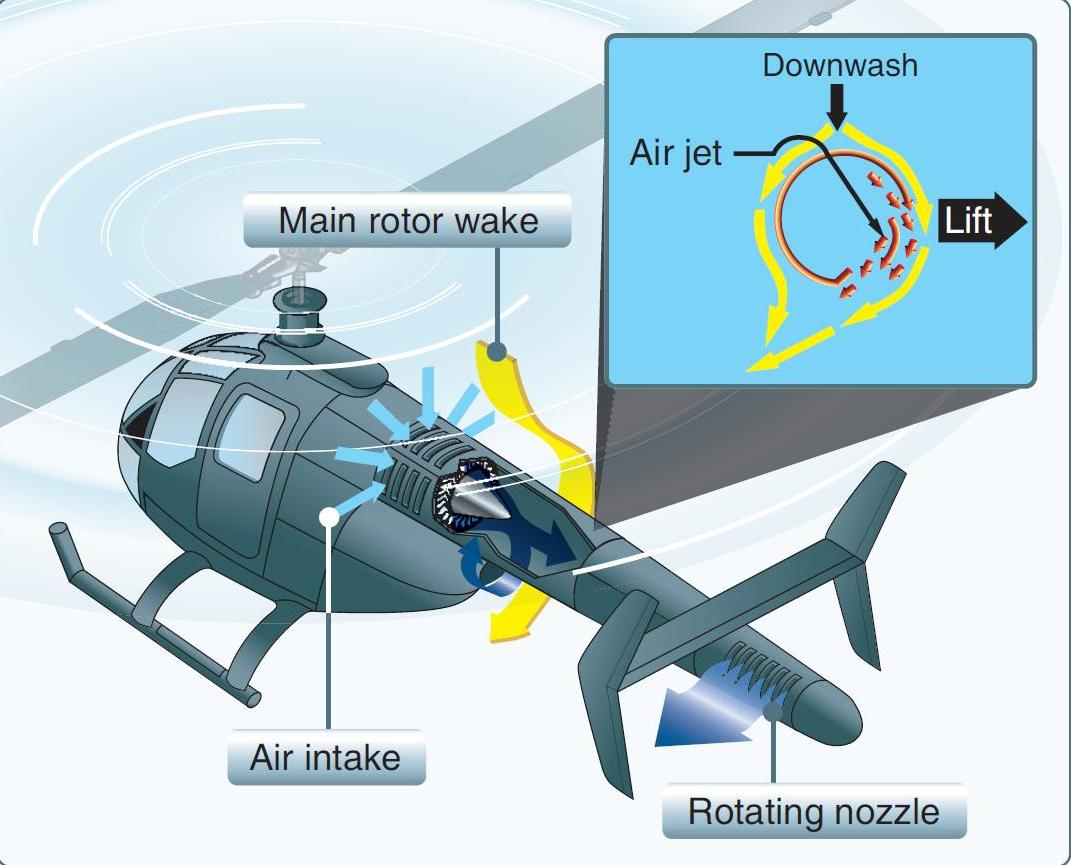
\includegraphics[height = 6cm]{Images/Literature/NOTAR}     
\caption{Image demonstrating the NOTAR system \cite{Heli}}
\label{IM_NOTAR}
\end{figure}

There have been many attempts at improving the standard helicopter design. These improvements have taken the form of adding rotors, designing hybrid aircraft and complex mechanical designs to harvest advantages of both the fixed wing and VTOL craft. Some have even tried to combine multiple features as Flanigan \cite{US7147182} did in his design of a tip-jet, compound, tilt rotor aircraft. 
In an attempt to keep the mechanical complexity to a minimum, not all configurations were investigated.

\subsection{Coaxial Rotors}
A coaxial configuration consists of two counter rotating blades located about the same centre of rotation that both use the same drive system. This eliminates the need for a tail rotor as the torque applied by both rotors cancel each other out, as shown in figure \ref{IM_Coaxial}\footnote{Image Taken from www.simhq.com}.  

\begin{figure}[H]
\centering
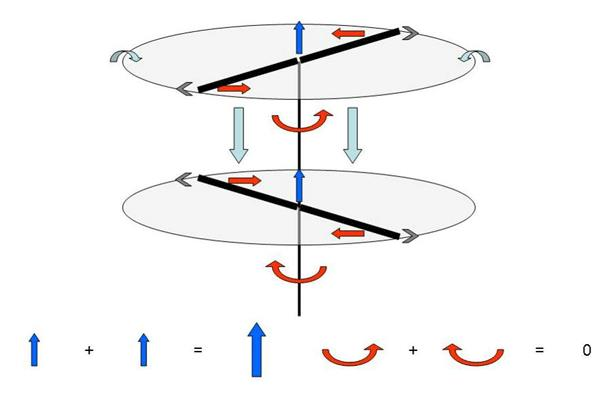
\includegraphics[height = 6cm]{Images/Literature/Coaxial}     
\caption{A standard Coaxial rotor set up and the induced forces}
\label{IM_Coaxial}
\end{figure}

Since half of the bottom blade is working in the top blades slip stream it will have a higher $v_0$ and therefore a larger $v_i$, which according to equation \eqref{EQ_ThrustBasic} will induce a larger thrust, relating to high values of efficiency and disk loading. Localising the blades around a single point also helps with the geometry of the craft as it is a more compact design. With no modifications and only using fixed pitched rotors, this platform will only give yaw and over all thrust control. Bohorquez et al in \cite{Bohorquez} attempted a number of lateral control methods, eventually settling on aerodynamic flaps to control the flow of the downwash, that and other methods are shown in figure \ref{IM_Coaxial_Variations}. Briod et all also used the same set up in his team's design of the Gimball \cite{Briod2012}.
 
\begin{figure}[H]
	\centering
	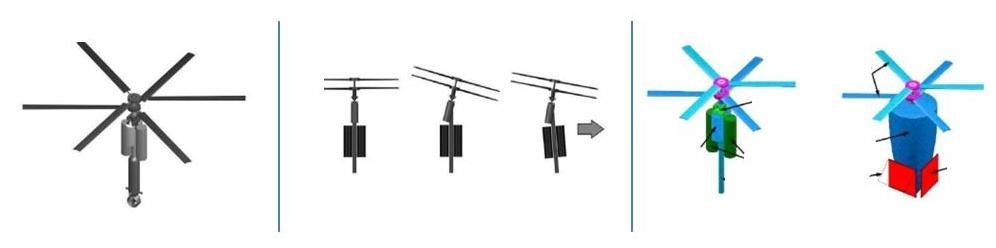
\includegraphics[height = 3cm]{Images/Literature/Coaxial_Configs}     
	\caption{Different methods of lateral control in a Coaxial MAV (Adapted from \cite{Bohorquez})}
	\label{IM_Coaxial_Variations}
\end{figure}

The control flaps are the most common used form of lateral control for small coaxial MAVs. They introduce little mechanical complexity and do not require excessive power to use. The flaps do however decrease efficiency of the system, but if designed correctly should only influence the system while being used. For hover and vertical flight the impact will be negligible. As a control surface the flap is quite rudimentary and will require some more advanced control methods as well as in depth testing to obtain smooth flight transitions. Due to its compactness the design can have considerable manoeuvrability if the control algorithms are designed effectively. Each flap will require an actuator, this will increase total weight, power consumption and required mechanics. 
\todo[inline]{Include Johnson's Calulations that states how much efficeincy is lost due to overlap}

\subsection{Tandem Rotors}

A tandem rotorcraft is sometimes referred to as a dual rotor, as it consists of two blades to generate thrust and to decrease disk loading and increase the lift capacity. In a tandem configuration the blades sit in the front and the rear of the craft, generally with a slight overlap. Tandems are often used in applications that require heavier loads than the traditional rotorcraft can effectively offer. A tandem configuration is demonstrated in figure \ref{IM_Tandem}\footnote{(Taken from \cite{Bee})}, the blades spin in opposite directions to counteract the other one's rotational torque. Pitch and Yaw control are readily available through manipulation of the rotor speeds, while roll control are not as easily accomplished with this design and generally require variable pitch rotors \cite{Oh2005}. Using two smaller blades also decreases the effects of interferences such as gusts on the craft, although a tandem helicopter has the problem of its rear rotor being influenced by the wake of the front rotor\footnote{In the case where the rotors overlap} \cite{Camrad1}. 

\begin{figure}[H]
\centering
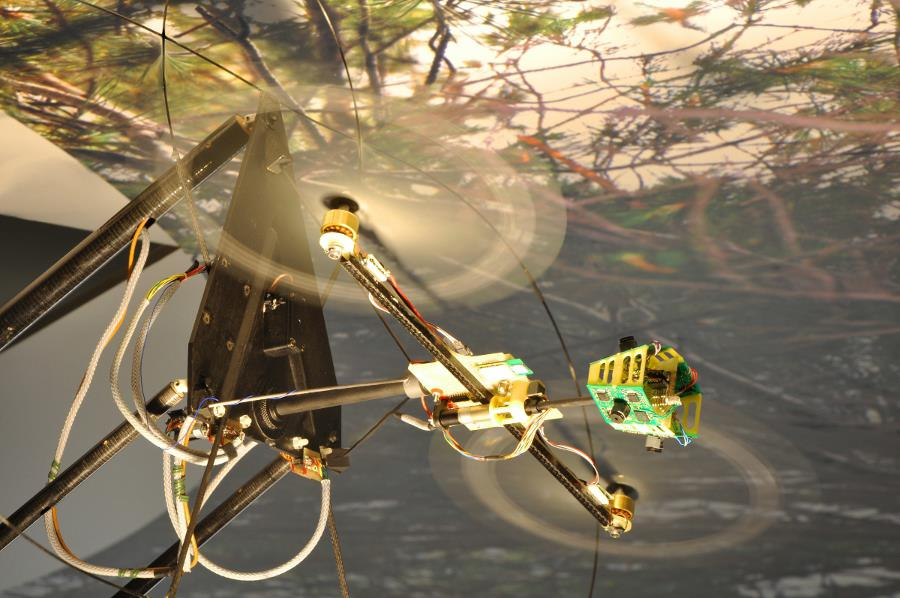
\includegraphics[height = 6cm]{Images/Literature/TandemBEE}     
\caption{The BeeRotor robot demonstrating a Tandem rotor set up in a MAV \cite{Bee}}
\label{IM_Tandem}
\end{figure}


As described in equation \eqref{EQ_ElectricalPowerThrust} the thrust of the system increases slower than the electrical power input into the system. In a standard configuration, doubling the electrical power would only increase the thrust by a factor of $\approx 1.587$. Where as doubling the amount of rotors being driven will double both the thrust and the electrical power. This gives the tandem arrangement the capability of lifting heavier loads with relatively low power consumption, as well as demonstrating low power consumption for hover and slow translatory flight. Having twin blades does increase the size of the craft, but the elimination of the tail rotor sees the size being similar to that of a classic helicopter.


\subsection{Multirotor Designs}

Drones have joined other remote controlled vehicles in the world of hobbyists. Of all the different designs the multirotor is the most popular. Through discussions with drone designers and aerial photographers, the four rotor design is generally chosen due to its incredible stability and manoeuvrability. Similar to the tandem, the quad has very good disk loading and thus can be used to lift heavy loads, there are even products that have 8 rotors to seriously increase the payload capability. This does however relate to a more power hungry system and a less efficient hover.

As shown in figure \ref{IM_CounterBlades}\footnote{(Taken from \cite{ThrustCritical})}, a quad rotor consists of two pairs of counter rotating propellers. Each shaft will be driven by its own motor and unlike the flaps in a coaxial system, every motor in a quadcopter attributes to the lift vector. Having the freedom to control each blade independently gives the pilot advanced manoeuvrability, with minimal mechanical complexities. This also reduces the complexity of the control algorithms as six degrees of freedom can be obtained by simply adjusting the speed of the motors, the multirotor can even rotate on the spot without any change in altitude \cite{ThrustCritical}. Besides the poor hover efficiency, the biggest downside of the multirotor designs is their size and weight. Each blade requires a drive system and space to rotate without interference.

\begin{figure}[H]
\centering
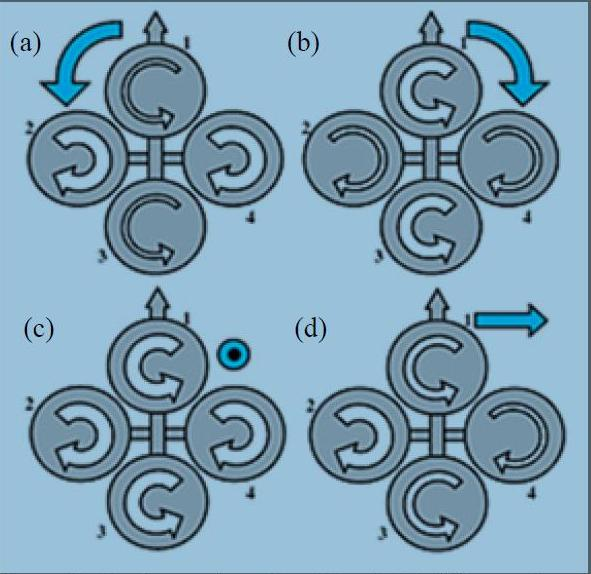
\includegraphics[height =6cm]{Images/Literature/QuadBlades}
\caption{Quadrotor configuration \cite{ThrustCritical}}
\label{IM_CounterBlades}
\end{figure}



\subsection{Tilt Rotors}

A tilt rotor is a very sophisticated system that attempts to harness the benefits of both the fixed and rotor wing aircraft. With the addition of a pivoting axis for each blade the craft has the forward flying speeds of a fixed wing craft while still being able to take off an land vertically like a rotorcraft. The tilt rotor's major downfall is related to the required highly complex and intricate mechanical design \cite{RotorConfig}.
 
VTOL applications require a larger blade to decrease the disk loading, while in forward flight a smaller diameter blade is desired to increase the efficiency of propulsion. Hager \cite{US6030177} developed a telescopic system that transforms the blades to get the optimal benefits out of each configuration, shown in figure \ref{IM_TiltRotor}\footnote{(Taken from \cite{Heli})}. These and other improvements have established the tilt rotor as a  competitive design in the field of aeronautic transportation \cite{RotorConfig}.

\begin{figure}[H]
\centering
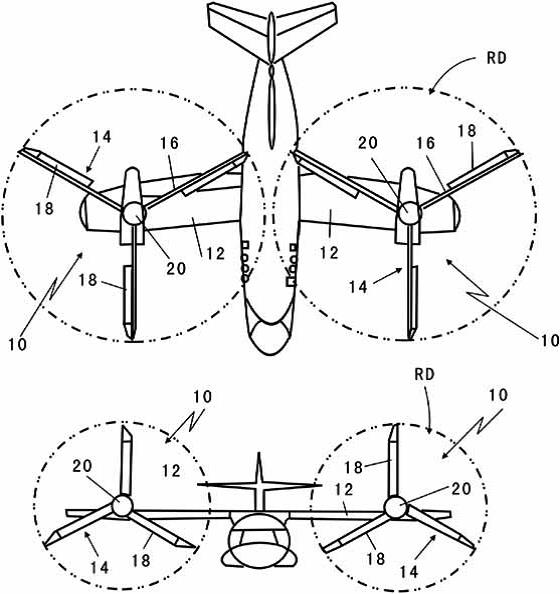
\includegraphics[height = 6cm]{Images/Literature/TiltRotor}     
\caption{Hager's design for a telescopic tilt rotor system \cite{Heli}}
\label{IM_TiltRotor}
\end{figure}


\section{Rotorcraft Flight Dynamics}

The flight dynamics of any rotorcraft can be  a complicated problem. This section will discuss some of the methods and issues pertaining to modelling these dynamics. Most of the discussion will surround multirotors, specifically quadrotors, as the majority of the literature is based on these designs \cite{Luukkonen, RealTime, Pounds2006, Hoffmann}. Due to the mechanical complexity of swashplate designs, the discussion is assuming a fixed pitched rotor set up. 

Before control laws can be applied there must be a dynamic model of the craft. To create the model there needs to be a good understanding of the craft dynamics as well as the mathematical methods for creating the appropriate equations. A brief introduction to rigid body dynamics is done and is followed by an in depth talk into modelling rotorcraft for the general case. After the model can be obtained mathematically it is important to discuss the physical implementation of obtaining the data, and the various instrumentation required. Unfortunately its very rare to have a flying environment that is void of disturbances, for this fact the section is ended off with a discussion about the various disturbances that effect the flight dynamics of any rotorcraft.

\subsection{Mass Model and the Inertia Tensor}
In any aerial vehicle mass is always an important design criterion. Every aspect of the platform must be designed to be the lightest it possibly can. Having a light weight craft is one part of the design criterion, another would be ensuring that the weight is geometrically spread out correctly, as well as functionally distributed appropriately. The table below was adapted from \cite{NewMAV} and demonstrates the latter point better. Depending on the different criteria for the craft, different functional blocks will be allocated a certain percentage of weight. For example if the user would like a longer flight time, a higher percentage would be given to the power source and possibly less to the external payload. Generating a good mass model before designing helps better understand the requirements for the craft and could be a deciding factor in the construction.

\begin{table}[H]
\centering
\begin{tabular}{l | c | c | c | c}

Component 					& 0.3kg & 1.8kg & 3.7kg\\
\hline\hline
Rotor System 				& 11.0 & 11.2 & 13.9\\
Tailboom Assembly 		& 8.0 & 9.1 & 7.8\\
Main Rotor Motor 			& 15.4 & 10.5 & 8.1\\
Fuselage/Structure 			& 7.0 &  15.1 & 12.0\\
Main Transmission 			& 2.0 &  3.4 & 3.4\\
Landing Gear 				& 2.3 &  3.4 & 2.9\\
Control System 				& 5.7 & 18.3 & 9.3\\
Avionics 						& 29.4 &  2.4 & 1.6\\
Power Source 				& 19.2 & 26.6 & 41.0\\

\end{tabular}
\caption{MAV Weight Data (Adapted from \cite{NewMAV})}
\end{table}

It was also mentioned that the weight needs to be geometrically positioned correctly, the point of this would be to create as much symmetry in the craft as possible. If this is done correctly the principle axes of inertia will align very closely with the body of the craft, simplifying calculations later on and helping find and define the principle axes. The inertia tensor is a matrix that is a representation of a rigid body's resistance to movements in 3D space, this is obviously crucial since the application is to move a body through 3D space! For the general case the inertia tensor takes the form as shown in equation \eqref{EQ_InertiaTensor}. The inertia tensor is very dependant on a craft's symmetry, and is symmetric itself. In other words, $I_{xy} = I_{yx}$, $I_{xz} = I_{zx}$ and $I_{zy} = I_{yz}$ and therefore if a craft is symmetric about the y axis (x = 0), then $I_{xy} = I_{yx} = 0 = I_{xz} = I_{zx}$ \cite{Luukkonen, MiniFlying}.

\begin{equation}
\label{EQ_InertiaTensor}
\textbf{I} = 
\begin{bmatrix}
I_{xx}	& -I_{xy} & -I_{xz}\\
-I_{yx}	& I_{yy}	& -I_{yz}\\
-I_{zx}	& -I_{zy}	& I_{zz}\\
\end{bmatrix}
\end{equation}


\subsection{Coordinate System}
As mentioned previously, there are six degrees of freedom (DOF) in 3D space, three of them translational and three of them rotational. With a quadcopter, 4 of these degrees of freedom are primary and 2 of them are secondary, being formed by combinations of the primary 4. Generally three dimensional space is modelled in terms of the three orthogonal axes x, y and z; where x and y are lateral movements and the z axis is the vertical movement with gravity being a purely negative z component. These axes will be referred to as the inertial frame and they are relative to the ground and gravity. Now of course the vehicle will not always be perfectly aligned with this frame, for this reason a second frame is defined and refers to the axes that line up with the body of the craft. It is thus named the body frame, these planes will alter as the craft moves around in space. Figure \ref{IM_Frames} visually demonstrates the relationship between the two frames. 

\begin{figure}[H]
\centering
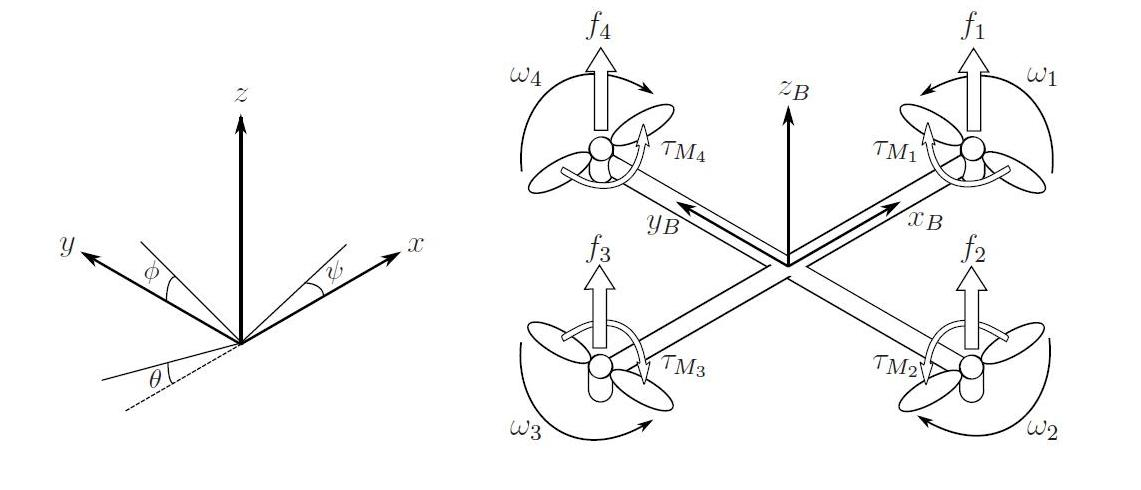
\includegraphics[height = 6cm]{Images/Literature/Frames.jpg}     
\caption{The body and inertial frames of a rotorcraft (Taken from \cite{Luukkonen})}
\label{IM_Frames}
\end{figure}

As shown they are separated by the roll ($\phi$), pitch ($\theta$) and yaw ($\psi$) angles of the craft, which relate to a rotation about the x, y and z axis respectively. These angles are the Euler angles of the rotation and according to Euler's theory, any two varying coordinate axes can be related to one another by a single rotational matrix. In the case of rotating from the body to the inertial frame, the matrix takes the form as shown in equation \eqref{EQ_RotationMatrix} \cite{Luukkonen} where $C_x = \cos(x)$ and $S_x = \sin(x)$. The matrix is also orthogonal, which means that $\textbf{R}^{-1} = \textbf{R}^T$, which would be the rotation from the inertial frame to the body frame \cite{Luukkonen, MiniFlying}.

\begin{equation}
\label{EQ_RotationMatrix}
\textbf{R} = 
\begin{bmatrix}
C_\psi C_\theta   	& C_\psi S_\theta S_\phi - S_\psi C_\phi & C_\psi S_\theta C_\phi + S_\psi S_\phi \\
S_\psi C_\theta   	& S_\psi S_\theta S_\phi + C_\psi C_\phi & S_\psi S_\theta C_\phi - C_\psi S_\phi\\
-S_\theta   		& C_\theta S_\phi & C_\theta C_\phi  \\
\end{bmatrix}
\end{equation}

Therefore if the yaw, roll and pitch angles are known, the angular position of the craft can be calculated with respect to the ground (or the inertial frame). The lateral position will be a combination of x, y and z points in the inertial frame. The naming scheme used in this paper is the same that is seen used by Castillo et al in \cite{MiniFlying, RealTime} with some variations from Luukkonen \cite{Luukkonen} and Carrilo et al \cite{Modelling}. It describes the position of the centre of mass as the value $\boldsymbol{\xi}$ while $\boldsymbol{\eta}$ represents the orientation of the craft in terms of the Euler angles, both numerical representations are shown below. The vector \textbf{\textit{q}} is the culmination of the previous data points to give one complete, descriptive vector for the inertia frame.

\begin{eqnarray}
\boldsymbol{\xi}= 
\begin{bmatrix}
x\\
y\\
z
\end{bmatrix}&
\boldsymbol{\eta} = 
\begin{bmatrix}
\phi\\
\theta\\
\psi
\end{bmatrix}& 
\textbf{\textit{q}} = 
\begin{bmatrix}
\boldsymbol{\xi}\\
\boldsymbol{\eta}
\end{bmatrix}
\label{EQ_InertiaFrame}
\end{eqnarray}

As described above, values in the body frame can be represented in the inertia frame via the rotation matrix $\textbf{R}$, and likewise values in the inertia frame can be represented in the body frame through a rotation of $\textbf{R}^{-1} = \textbf{R}^T$. The body coordinate system takes the same form as the inertia frame, just with a different naming scheme. For simplicity, all vector components relative to the body frame will be followed with a B subscript, so in the inertia frame the components will be the familiar $\hat{\textbf{i}}$, $\hat{\textbf{j}}$ and $\hat{\textbf{k}}$ and the components relative to the body frame will be shown as $\hat{\textbf{i}}_B$, $\hat{\textbf{j}_B}$ and $\hat{\textbf{k}}_B$.

It makes sense that the global position and orientation of the craft be described in the inertia frame, since generally those values will be discussed relative to that frame. The velocities however will generally be discussed relative to the body frame. Since there is now a simple relationship between the two frames, it is possible to assess different parameters in the different frames, as long as when they are discussed together they are both converted to the same coordinate axes. Equation \eqref{EQ_BodyFrameSpeeds} represents the translational speeds as $\textbf{V}_B$ and the rotational speeds as $\boldsymbol{\Omega}_B$, both of which are relative to the body frame.

\begin{eqnarray}
\textbf{V}_B = 
\begin{bmatrix}
V_{x_B}\\
V_{y_B}\\
V_{z_B}
\end{bmatrix}&
\boldsymbol{\Omega}_B = 
\begin{bmatrix}
p\\
q\\
r
\end{bmatrix}
\label{EQ_BodyFrameSpeeds}
\end{eqnarray}

Rotation matrix $\textbf{R}$ is used to describe variables measured in the body frame to the inertia frame. As seen in Luukkonen \cite{Luukkonen} the general case for velocities will require a rotation from the inertial frame to the body frame. That is done with a rotation $\textbf{\textit{W}}_\eta$, with the inverse being a rotation for speeds taken in the body frame to the inertial frame. Therefore $\boldsymbol{\Omega}_B = \textbf{\textit{W}}_\eta \times \dot{\boldsymbol{\eta}}$ and $\dot{\boldsymbol{\eta}} = {\textbf{\textit{W}}_\eta}^{-1} \times \boldsymbol{\Omega}_B$. Where $\textbf{\textit{W}}_\eta$ is represented by the matrix shown in equation \ref{EQ_VelocityRotation} \cite{Luukkonen, Modelling}.

\begin{equation}
{\textbf{\textit{W}}_\eta} = 
\begin{bmatrix}
1 & 0 & -S_\theta\\
0 & C_\phi & C_\theta S_\phi\\
0 & -S_\theta & C_\theta C_\phi
\end{bmatrix}
\label{EQ_VelocityRotation}
\end{equation}

In summation, the local coordinates of the craft will be measured according to the inertial axes and can be translated to the body frame through the rotation $\textbf{R}$. The coordinates are represented by the variable $\textbf{\textit{q}}$. Which encompasses the lateral position ($\boldsymbol{\xi}$) and the rotational position, or orientation, ($\boldsymbol{\eta}$).The velocities of the craft however, will be measured relative to the body frame and can be converted to the inertial frame using the rotation $\textbf{\textit{W}}_\eta$. The velocities are also composed of translational ($\textbf{V}_B$) as well as rotational components ($\boldsymbol{\Omega}_B$).

\subsection{Dynamic Flight Model}

The general coordinates of a system, like the ones described above, is the smallest set of parameters that can unambiguously describe the configuration of that system. The number of variables used will equal to the number of degrees of freedom \cite{MIT}. 
Since the vector \textbf{\textit{q}} gives an absolute position of the craft, the derivative, $\dot{\textbf{\textit{q}}}$, should represent the speeds with the double derivative, $\ddot{\textbf{\textit{q}}}$, giving accelerations. The form of the problem allows the use of Lagrangian mechanics and formulae to solve for the forces \cite{MIT, MiniFlying}. Since the system can be considered as  a rigid body, normal Newtonian mechanics can be used to solve the problem and will also use the Euler angles described above \cite{Luukkonen, Modelling}. Both methods are briefly discussed, using a standard quadcopter as an example. Before the models can be generated a discussion must be had on the forces involved.  Figure \ref{IM_Frames} is used as a descriptive aid for the following section.


\subsubsection{Translational Forces}
For a quadcopter all the forces are generated by the 4 rotors. Simplifying the system that the rotors are fixed-pitched entails that the applied forces only have a tangible $\hat{\textbf{k}}_B$ component.

\begin{eqnarray}
\textbf{F}_B = (f_1 + f_2 + f_3 + f_4)\hat{\textbf{k}}_B & where & f_i = k_i {\omega_i}^2
\label{EQ_Translational}
\end{eqnarray}

The individual force components ($f_i$) can be calculated using a constant ($k_i$) and the angular rotor speed ($\omega_i$) \cite{RealTime}. Now that the forces are expressed in the body frame, they can be converted into the inertial frame through the rotation $R^T$. Therefore $\textbf{F}_\xi = R^T \textbf{F}_B$.

\subsubsection{Rotational Forces}
As said above, all of the controlled forces are generated by the rotors, this includes the moments. The traditional variations in angular position that the quadcopter experiences are all created by independently varying the speed of the motors. These moments can be mathematically expressed as shown in \ref{EQ_moments}, $l$ is the distance from the centre of the rotor to the centre of gravity. \cite{Modelling}

\begin{eqnarray}
\tau_\psi = \sum_{1}^{4} \tau_{M_i};&
\tau_\theta = (f_2 - f_4)l_{4,2};&
\tau_\phi = (f_3 - f_1)l_{1,3}
\label{EQ_moments}
\end{eqnarray}

Effectively what the equations say is that if a there is an imbalance in the clockwise and counter-clockwise rotations, there will be an induced yaw moment ($\tau_\psi$). If differential commands are sent to geometrically opposite rotors, there will either be an induced pitch ($\tau_\theta$) or roll ($\tau_\phi$) moment, depending on how the frames are set up, this is demonstrated in figure \ref{IM_CounterBlades}.

\subsubsection{Accelerations Model}
Equations \ref{EQ_Translational} and \ref{EQ_moments} refer to the input forces, or control authority we have. To complete the model it is necessary to now understand how these inputs effect our global position \textbf{\textit{q}}. Using the Lagrangian in equation \ref{EQ_Lagrange} accelerations in the six DOF  can be solved for. Equation \ref{EQ_LagrangeAcceleration} shows the result of this mathematics and completes the model used by Castillo et al \cite{MiniFlying, RealTime}. Each output, or degree of freedom, is now related to one of the input forces.

\begin{eqnarray}
\label{EQ_LagrangeAcceleration}
m\ddot{x} &=& -\lvert \textbf{F}_B \rvert\sin\theta\\
m\ddot{y} &=& \lvert \textbf{F}_B \rvert\cos\theta\sin\phi\\
m\ddot{z} &=& \lvert \textbf{F}_B \rvert\cos\theta\cos\phi - mg\\
\ddot{\psi} &=& \tilde{\tau}_\psi\\
\ddot{\theta} &=& \tilde{\tau}_\theta\\
\ddot{\phi} &=& \tilde{\tau}_\phi
\end{eqnarray}

Although Castillo's model has obtained some positive results, his model is simplified with decisions such as neglecting the Coriolis effects from the rotors. This simplification can be seen by the addition of the tilde above the torque symbols in \ref{EQ_LagrangeAcceleration} and  can be seen in numerous readings \cite{MiniFlying, RealTime, Modelling}. Even with these faults the model is a good basis for modelling a rotorcraft. Luukkonen in \cite{Luukkonen} decided not to neglect the Coriolis effects and added an additional term into his model, $\textbf{C}(\boldsymbol{\eta}, \dot{\boldsymbol{\eta}})$, which is a three by three matrix holding all the Coriolis values. 

\begin{eqnarray}
\label{EQ_LagrangeAccelerationCoriolis}
\boldsymbol{\tau} = \textbf{C}(\boldsymbol{\eta}, \dot{\boldsymbol{\eta}})\dot{\boldsymbol{\eta}} + \mathbb{J}\tilde{\boldsymbol{\tau}} & where & \tilde{\boldsymbol{\tau}} = \begin{bmatrix}
\tilde{\tau}_\phi\\
\tilde{\tau}_\theta\\
\tilde{\tau}_\psi
\end{bmatrix}
\end{eqnarray}


\subsubsection{Euler-Lagrangian Approach}
The Lagrange model is repeatedly used in generating models for rigid body dynamics \cite{MIT, MiniFlying, Luukkonen, RealTime}. There are a few benefits to using this model opposed to the standard Newtonian approach. The Lagrange approach produces as many equations as their are degrees of freedom, in a system where there are 6 degrees of freedom this can become pertinent to solving the model. Using the Lagrangian automatically eliminates non-contributing forces and it will take advantage of the now formulated general coordinate system described above \cite{MIT}.

The Lagrangian uses the energy conversation principles to obtain a formula for the forces acting in a system. The Lagrangian function is the difference between the kinetic (\textbf{T}) and potential energies (\textbf{U}), it takes it simplest form as $ \textbf{L}( \textbf{\textit{q}}, \ddot{ \textbf{\textit{q}}}) = \textbf{T} - \textbf{U}$, equation \eqref{EQ_Lagrange} is the expanded equation. 
Where the kinetic energy is broken into two parts, rotational and translational. The major contributing potential energy takes the form of $\textbf{U} = (mgz) \hat{\textbf{k}}$ and it represents the gravitational potential of the craft. The kinetic energies can be represented as $\textbf{T}_{rot} = \dfrac{1}{2} \dot{\boldsymbol{\eta}}^T \mathbb{J} \dot{\boldsymbol{\eta}}$ and $\textbf{T}_{trans} = \dfrac{m}{2} \dot{\boldsymbol{\xi}}^T \dot{\boldsymbol{\xi}}$. Where $\mathbb{J}$ is the inertia tensor in terms of $\boldsymbol{\eta}$ and $\mathbb{J} = {\textbf{\textit{W}}_\eta}^T \textbf{I} \textbf{\textit{W}}_\eta$ \cite{Luukkonen, Modelling}.

\begin{eqnarray}
\textbf{L}( \textbf{\textit{q}}, \ddot{\textbf{\textit{q}}}) =  \dfrac{1}{2} \dot{\boldsymbol{\eta}}^T \mathbb{J} \dot{\boldsymbol{\eta}} + \dfrac{m}{2} \dot{\boldsymbol{\xi}}^T \dot{\boldsymbol{\xi}} - mgz
\label{EQ_Lagrange}
\end{eqnarray}

The actual model is then based on the standard form of the Euler-Lagrange equations is shown in equation \eqref{EQ_EulerLagrange} below.

\begin{equation}
\dfrac{d}{dt} \dfrac{\partial \textbf{L}}{\partial \dot{\textbf{\textit{q}}}} -  \dfrac{\partial \textbf{L}}{\partial \textbf{\textit{q}}}= \textbf{F}
\label{EQ_EulerLagrange}
\end{equation}

Where $\textbf{F}$ is the culmination of all the forces being experienced by the craft in relation to the inertial frame. Since the Lagrangian accounts for all the degrees of freedom, $\textbf{F}$ encompasses both the translational forces ($\textbf{F}_\xi$) as well as the rotational moments ($\boldsymbol{\tau}$), $\textbf{F} = (\textbf{F}_\xi, \boldsymbol{\tau})$. It can be seen from equation \eqref{EQ_Lagrange} that these two forces can be observed independently from each other \cite{RealTime}.

\subsubsection{Newton-Euler Method}
The method described above involves using the Lagrangian definition to obtain the equations of motion. Another method is to keep the same coordinate system using Euler's methods and then applying Newton's laws of motion to obtain the model. Either approach will yield a model and will depend on personal preference for a decision. Newton's method is more familiar to some and does not involve the more complicated Lagrangian mathematics. The downfall is the coordinate system derived above is not fully taken advantage of, and the mathematical model can feel more complicated since non-contributing forces are still considered. The Newton model does however allow elimination of certain disturbances due to referencing from different frames. 
In \cite{Luukkonen, Modelling} both approaches are analysed an compared and it is shown that both approaches obtain the same model.

When using the Newton-Euler method, it is of crucial importance to remember which reference frame is being worked with. Ideally an absolute value for accelerations is desired i.e using the inertial frame as a reference. To begin, consider the forces required to accelerate the mass $m\textbf{V}_B$ as well as to counter the centrifugal force $\boldsymbol{\Omega}_B \times (m\textbf{V}_B)$. These forces take the form of the applied thrust $\textbf{F}_B$ as well as the gravity component, a rotation is needed to place the gravitational force in the body frame resulting in a force of $\textbf{R}^T \textbf{G}$ \cite{Luukkonen}. Relating these via Newton's 2nd law of motion, \eqref{EQ_EulerNewton} can be obtained.

\begin{equation}
m\textbf{V}_B + \boldsymbol{\Omega}_B \times (m\textbf{V}_B) = \textbf{F}_B + \textbf{R}^T \textbf{G}
\label{EQ_EulerNewton}
\end{equation}

Since centrifugal forces are eliminated when using the inertial frame, \eqref{EQ_EulerNewton} can be used to obtain  \eqref{EQ_EulerNewtonInertial} which can also be represented in matrix notation, as shown in \eqref{EQ_EulerNewtonInertialMatrix} \cite{Luukkonen}. 

\begin{equation}
m\ddot{\xi}  = \textbf{R}\textbf{F}_B + \textbf{G}
\label{EQ_EulerNewtonInertial}
\end{equation}

\begin{equation}
\begin{bmatrix} \ddot{x}\\ \ddot{y}\\ \ddot{z} \end{bmatrix} = -g\begin{bmatrix} 0\\ 0\\ 1 \end{bmatrix} + \frac{\textbf{F}_B}{m} \begin{bmatrix}
C_\psi S_\theta C_\phi + S_\psi S_\phi\\
S_\psi S_\theta C_\phi - C_\psi S_\phi\\
C_\theta C_\phi
\end{bmatrix}
\label{EQ_EulerNewtonInertialMatrix}
\end{equation}

As for the rotational velocities, the external torque ($\boldsymbol{\tau}$) must be big enough to provide the inertia ($\textbf{I}$) with the required acceleration ($\boldsymbol{\dot{\Omega}}_B$), while overcoming the centripetal ($\boldsymbol{\Omega}_B \times \textbf{I}\boldsymbol{\Omega}_B$) and the gyroscopic forces ($\boldsymbol{\Gamma}$). Equation \eqref{EQ_EulerNewtonRotation} is the mathematical representation of the applied torque. Equation \eqref{EQ_EulerNewtonRotationMatrix} is the matrix where the accelerations have been solved for.

\begin{equation}
\textbf{I} {\boldsymbol{\dot{\Omega}_B}} + \boldsymbol{\Omega}_B \times \textbf{I}\boldsymbol{\Omega}_B + \boldsymbol{\Gamma} = \boldsymbol{\tau}
\label{EQ_EulerNewtonRotation}
\end{equation}

\begin{equation}
\begin{bmatrix}\dot{p}\\ \dot{q} \\ \dot{r} \end{bmatrix} = \begin{bmatrix} I_{yy} - I_{zz}qr/I_{xx}\\ I_{zz} - I_{xx}pr/I_{yy}\\ I_{xx} - I_{yy}pq/I_{zz} \end{bmatrix} - I_r \begin{bmatrix} q/I_{xx}\\ -p/I_{yy} \\ 0 \end{bmatrix} \omega_\Gamma + \begin{bmatrix}\tau_\phi/I_{xx} \\ \tau_\theta/I_{yy} \\ \tau_\psi/I_{zz}  \end{bmatrix}
\label{EQ_EulerNewtonRotationMatrix}
\end{equation}

Where $\omega_\Gamma = \omega_1 - \omega_2 + \omega_3 - \omega_4$ \cite{Luukkonen}.

\subsection{Disturbances}
The acceleration model developed by Castillo et al \cite{MiniFlying} only considers forces generated by pilot inputs to the system. Most readings that involve rotor dynamics will include a section about disturbances, or aerodynamic effects \cite{Hoffmann, Pounds2006, Luukkonen, NearWall} since they also can severely effect the craft dynamics. Most of the aerodynamic forces are only pertinent at higher velocities, as they are created through an increase in velocity of the air speed. In the case of Luukkonen \cite{Luukkonen}, he addresses the disturbances but omits them from the model since they are negligible at the speeds his craft would be travelling.

\subsubsection{Drag}
Drag is a resistive force whose quantity is relative to the speed of the object in question and is always in the direction opposing the motion. It can be seen as the friction forces created by the air. Equation \ref{EQ_Drag} quantifies the effect of drag. Luukkonen \cite{Luukkonen} uses a simple matrix to include the drag effects in his acceleration model, simply subtracting the components of drag from each acceleration component. As seen from the equation, the effect of drag can be reduced through mechanical design, by reducing the area of the plane facing towards the direction of the motion. 

Since the rotors spin at such high speeds they also experience high levels of drag, the effect of rotor drag is seen as a drop in efficiency as it constantly acts against the motors. Rotor drag is also responsible for other random disturbances in the craft dynamics.

\subsubsection{Blade Flapping}
It was mentioned earlier in the text about the issue with the difference in tip velocities for the advancing and the retreating case. Not only is it a total speed limitation, it also creates a disturbance called blade flapping. Figure \ref{IM_BladeFlapping}\footnote{Taken from (http://www.dynamicflight.com/aerodynamics/flapping/) and \cite{Hoffmann}} shows two different views of the effect as a visual aid in this subsection. 

The difference in velocity of the two edges creates a cyclical variance in angle of attack, similar to an uncontrolled version of cyclic control used in the traditional helicopter. This varying angle of attack creates a dissymmetry of lift that causes instability in the craft and a flapping motion of the rotors. The blades will flap up and down in a single revolution creating a very fast disturbance equations, for this reason they can be seen as instantaneous functions, and the timing of the flapping does not need to be considered \cite{Pounds2006}.

As described in \cite{Hoffmann, Pounds2006}, this variance in angle of attack effectively creates a new frame which lines up with the now angled rotors. Angle $a_{1s}$ is the deflection from the rotor normal and is the modification variable of the of thrust components. This results in a decrease in the $\hat{\textbf{\textit{k}}}_B$ component of thrust equivalent to $\cos (a_{1s})$. The lateral component of this force is cancelled out by the symmetry of the quadcopter, as well as the moment it produces around the rotor \cite{Hoffmann}.

\begin{figure}[H]
\centering
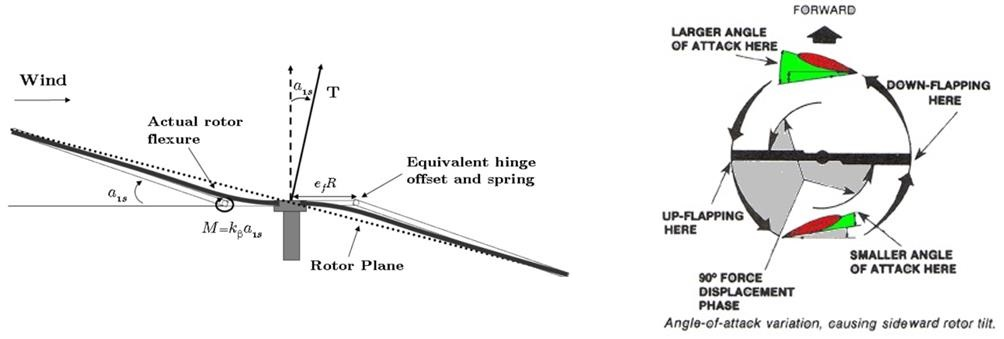
\includegraphics[height = 5cm]{Images/Literature/BladeFlapping3}     
\caption{Qualitative effects of blade flapping.}
\label{IM_BladeFlapping}
\end{figure}

Blade flapping will not be apparent when the craft is in a state of hover and there is no wind. Flying the quadcopter effectively generates wind lateral to the rotors and this causes the change in speeds of the rotor tips. The problem is generated by the non zero airflow through the rotors. Airflow disruption in general will cause quantifiable effects to the rotorcraft and should definitely be included in the model.

\subsubsection{Airflow Disruption}
Airflow can be an ambiguous phrase, since it is not always the air that is flowing, rather it could be labelled as relative airflow since that is what affects the dynamics of the craft. Airflow can be seen as the stream of air from $v_0$ to $v_i$ and then all the way down to $v_\infty$ similar to that shown in in figure \ref{IM_MomentumTheoryAirFlow} with naming scheme following figure \ref{IM_MomentumTheoryHover}. The three velocities are all linked through equation \ref{EQ_RotorVelocity} and equation \ref{EQ_ThrustMass} states that thrust is directly proportional to these velocities. It can be shown then that any deviation in these velocities will vary the thrust of the rotor in question. $v_0$ is only zero when the craft is in a state of pure hover, completely stationary, and there is no wind. Increasing the speed of the craft will increase the $v_0$ component creating a variation in the overall thrust, the same can be said for any condition that contains a tangible wind factor. 

Humidity and air density also play a significant role in rotor dynamics, although it is very unlikely that the air percentages will suddenly change, this must be considered when designing a craft for multiple climates and seasons.

The third airflow disruption that will be addressed is the effects that mechanical intrusions will have on the far wake velocity. In the design of STARMAC by Hoffmann et al \cite{Hoffmann} the frame was designed to be very configurable so that the effects of the mechanical design could be quantified. Originally the rotors were shrouded and quite close to the COG of the craft. The shrouds were a distance of 5\% rotor radius and when removed the yaw tracking improved from $\pm$10\textdegree to $\pm$3\textdegree. When not included in the dynamic model the obstruction in the air stream will cause lower and less stable values of thrust, affecting the stability of the model. 
When the rotors were located close to the centre of gravity they obtained some attitude disturbances that were eliminated by moving the rotors further away. It was also observed that any object that lies close to the rotor tip, created intense arbitrary disturbances and should be avoided. 

There is another disturbance that greatly affects the rotor performance called near ground or near wall effect and as the name stipulates, only occurs when the craft approaches a large immovable object.

\subsubsection{Near Ground Effect} \label{SSSECT_NearGroundEffect}
Robinson et al \cite{NearWall} created and validated a computational fluid dynamics mode to help quantify and understand the effects of near wall hovering for a traditional micro helicopter. The results of the study mainly focus on the rotor and thus will be very applicable to a collision resistant MAV regardless of the rotor configuration.

Figure \ref{IM_NearWall} is an image generated through the model and represents the velocities of the air stream descried above. Note how the no wall case represents, very closely the air flow described in figure \ref{IM_MomentumTheoryAirFlow} while the near wall case has some deviations. Effectively the velocities close to the wall are significantly less uniform than those that are away from the wall. This phenomenon is caused by the boundary layer created close to the wall. This asymmetry in the induced air stream creates reaction forces, the magnitude of which changes as the azimuth angle of the rotor changes. Since the rotors spin at such high velocities the force can be averaged to get a force component that only has tangible effects in the direction of the wall. The component parallel to the wall is not greatly affected as there is still a considerable amount of symmetry in that direction. Due to these reaction forces there is an induced moment that will reduce gradually as the rotor gets further away from the wall.  

\begin{figure}[H]
\centering
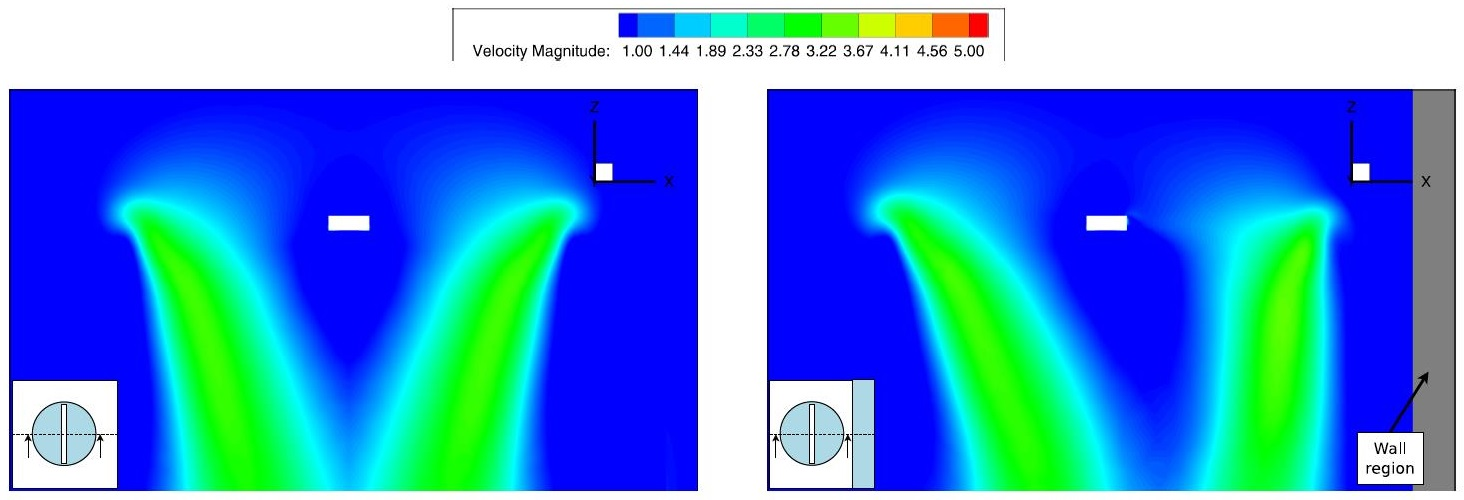
\includegraphics[height = 5cm]{Images/Literature/NearWall}     
\caption{Velocity components though the rotor for, no wall (left) and near wall (right) conditions (Taken from \cite{NearWall})}
\label{IM_NearWall}
\end{figure}

In \cite{NearWall}, Robinson et al used the script $c$ as their unit of measure for distance to the wall, $c$ is chord length of the airfoil. The graph shown in Figure \ref{IM_NearWallGraph} shows how the moment felt by the craft varies with the distance to the wall.

\begin{figure}[H]
\centering
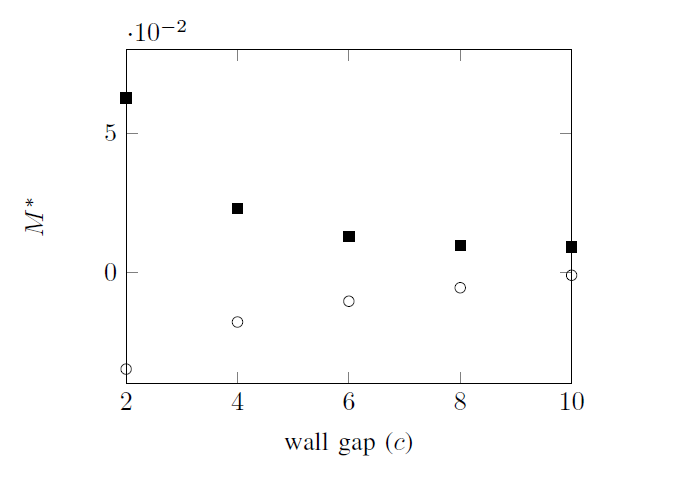
\includegraphics[height = 5cm]{Images/Literature/NearWallGraph}     
\caption{Graph showing relationship between distance from the wall and moment felt be the craft (Taken from \cite{NearWall})}
\label{IM_NearWallGraph}
\end{figure}

In \cite{NearWall} they conclude their paper by describing a proposed method of control which will be discussed further in the text.

\subsection{Instrumentation}
\todo[inline]{Incomplete}
In the final chapter of the book written by Castillo et al \cite{MiniFlying} there is a section on appropriate instrumentation for use in a MAV. The chapter includes devices such as a GPS and various other sensors and microcontrollers that can be added to a rotorcraft design. This section of the report will only address sensors that will aid in attitude and other movement measurements.

The most commonly used


\section{Methods for Control}
\todo[inline]{Incomplete}
\subsection{Stable Hover}
\subsection{Altitude Control}
\subsection{Attitude Control}
\subsubsection{Disturbance Observer}
\todo[inline]{\cite{NearWall} has awesome section on this}

\section{Collision Protection Techniques}
\todo[inline]{Need to decide if I should keep this in,l and in what format}
\cite{Klaptocz2013, Collision, Klaptocz2012, Briod2012, Daler2013, Klaptocz2010}
\subsection{Collision Avoidance}
%Not suitable for this application will still include some collision avoidance techniques
\subsection{Impact Resistance}
%Refer to impulse equations, Newtons's laws
%look at car designs
Impact resistance is a technique used by a variety of fields in the world today. Included in this is something as simple as the shocks or suspension in a car, they are designed to allow the automotive to withstand sudden impacts. Generally these techniques use a component that has some tangible spring constant.


\subsection{Rolling Cage}
\todo[inline]{Although a lot can be learnt from this design in terms of collision resistance, for the proposed end use case the design will not be pursued. The rolling cage design}